\documentclass[12pt,a4paper,toc=bibliographynumbered,toc=indenttextentries]{scrreprt}
\usepackage[utf8]{inputenc}
\usepackage[T1]{fontenc}
\usepackage{lmodern}
\usepackage{microtype}
\usepackage{setspace}
\usepackage[ngerman]{babel}
\usepackage{doi}
\usepackage{url}
\usepackage{ccicons}
\usepackage{graphicx}
\usepackage{caption}
\bibliographystyle{biolett}

\usepackage{orcidlink}

\author{Leonard Knegendorf}
% ORCID of the author: https://orcid.org/0000-0001-8469-1248
\title{FAIRE Publikation eines Beispieldatensatzes}

\begin{document}
	\begin{titlepage}
		\centering
		\textsc{\large{Hochschule Mannheim\\Master of Science\\Biomedizinische Informatik und Data Science\\Forschungsdatenmanagement (FDM)\\Prof. Dr. Dagmar Waltemath}}\par

		\vspace{3cm}
		\textbf{\huge{FAIRE Publikation eines Beispieldatensatzes\\}}\par
	
		\vspace{3cm}
		\textsc{\large{Hausarbeit}}\par
		
		
		\vfill
		vorgelegt von\par
		\textbf{Leonard Knegendorf~\orcidlink{0000-0001-8469-1248}}\par
		Hildesheim 2021
	\end{titlepage}

	
	\thispagestyle{empty}
	\mbox{}
	\vfill
	\begin{center}
	\begin{tabular}{|p{.9\textwidth}|}
	\ccbysa \bigskip\par\noindent
	\small{FAIRE Publikation eines Datensatzes von Leonard Knegendorf ist lizenziert unter einer \href{http://creativecommons.org/licenses/by-sa/4.0/}{Creative Commons Namensnennung - Weitergabe unter gleichen Bedingungen 4.0 International Lizenz}.\bigskip\bigskip\par\noindent
	Beruht auf dem Datensatz:\par
	\noindent Walonoski~J, Klaus~S, Granger~E, Hall~D, Gregorowicz~A, Neyapally~G, Watson~A, Eastman~J. 2020 Sythea\texttrademark~Novel coronavirus (COVID-19) model an synthetic data set.
	\newblock \emph{Intelligence-Based Medicine}~\textbf{1}, 1:100007. \newblock (\doi{10.1016/j.ibmed.2020.100007}).~\cite{10.1016/j.ibmed.2020.100007}\par\medskip
	Download unter:
	\url{https://storage.googleapis.com/synthea-public/10k_synthea_covid19_csv.zip}.}
	\end{tabular}
	\end{center}
	\thispagestyle{empty}
	\clearpage
	
	\thispagestyle{empty}
	\tableofcontents
	\clearpage
	
	\chapter{Einleitung}
	Das Ziel dieser Hausarbeit ist die Dokumentation des Prozesses zur "FAIRen Publikation" eines COVID--19 Beispieldatensatzes. Mit einer "FAIRen Publikation" ist im Zusammenhang dieser Arbeit eine nachhaltige und offene Publikation anhand der FAIR-Kriterien gemeint, welche 2016 durch Wilkinson \textit{et al.}~\cite{10.1038/sdata.2016.18} publiziert wurden und seitdem eine breite Anwendung im Feld des Datenmangements und zu einem der wichtigsten Standards geworden sind~\cite{10.1016/j.cels.2019.09.011}. \par
	Die FAIRe Publikation erfolgt anhand eines Beispielszenarios. Dieses beschreibt ein Forschungsvorhaben zur Untersuchung der Wirkung unterschiedlicher Medikationen auf die Behandlung von COVID-19 Patienten. Die Daten zu dieser Analyse entstammen drei Einzelstudien. Es sollen insbesondere Abhängigkeiten des Geschlechts und der Ethnie auf die Wirkung der Medikationen geprüft werden. Der Datensatz, der für diese Hausarbeit genutzt wird, basiert auf dem synthetischen COVID-19 Datensatz von Walonoski \textit{et al.}~\cite{10.1016/j.ibmed.2020.100007}, der mithilfe des Synthea Patientendatengenerators~\cite{10.1093/jamia/ocx079} erzeugt wurde. 
	Als erster Schritt, vor Beginn der Erstellung der eigentlichen Hausarbeit und der Bearbeitung des Datensatzes, erfolgte die Festlegung der Lizensierung. Die Wahl der Lizenz für die vorliegende Hausarbeit erfolgte mithilfe des \href{https://creativecommons.org/choose/}{Creative Commons License Chooser}. Anschließend wurde die System-Umgebung zur Dokumentation eingerichtet welche im Folgenden näher erläutert wird.
				
		\section{Beschreibung der System-Umgebung}
		Zu Beginn des Projektes wurde Wert auf die Einrichtung einer definierten System-Umgebung gelegt, in der die Bearbeitung des Datensatzes erfolgen kann.
		Die Versionskontrolle des bearbeiteten Datensatzes selbst erfolgt gemäß der Aufgabenstellung in einer FAIRDOMHub Sandbox. Bei FAIRDOMHub handelt es sich um ein Repositorium und eine Co-Working-Plattform die für Forschungsprojekte im Bereich der Systembiologie entwickelt wurde~\cite{10.1093/nar/gkw1032}. Der Datensatz wird im FAIRDOMHub in ein ISA Framework eingebettet, wie es im Grundsatz von Sansone \textit{et al.} vorgeschlagen wurde~\cite{10.1038/ng.1054}. Der Aufbau des ISA Frameworks erfolgt hierbei analog zum Framework, das durch Dagmar Waltemath und Sarah Braun für die Aufgabenstellung angelegt worden ist (\url{https://sandbox12.fairdomhub.org/investigations/12}). In der Benennung wird dem vorgegebenen Namen je ein Unterstrich und die Initialen LK angehängt, um das Framework nicht ausschließlich durch die SEEK ID von dem der Aufgabenstellung unterscheiden zu können. Die erste Version des Datensatzes wird durch eine Kopie des Datensatzes aus der Aufgabenstellung erzeugt, diese wird mit \textsf{Hausarbeit\_Datensatz\_COVID19\_LK\_v0.xlsx} benannt.\par  
		Die Texdokumentation der Bearbeitungsschritte erfolgt in einem \LaTeX{}-Dokument. Hierzu wurde zunächst ein GitHub-Repositorium erstellt, mithilfe dessen eine automatisierte Versionskontrolle der Projektdokumentation erfolgen kann (\url{https://github.com/lknegendorf/Master-BIDS-FDM_Hausarbeit}). Die Gliederung der Projektdokumentation gemäß der Aufgabenstellung wurde als erste Version der Textdokumentation in das Repositorium geladen. Darüber hinaus wurde eine tabellarische Übersicht der Dateistruktur und der Versionierung des GitHub-Repositoriums in dessen Wiki erstellt (\url{https://github.com/lknegendorf/Master-BIDS-FDM_Hausarbeit/wiki/%C3%9Cbersicht-%C3%BCber-Dateistruktur-und-Versionierung}).  
		
	\chapter{Bearbeitung der Aufgabenstellung}
		
		\section*{1. FAIR-Kriterien}
		Im Folgenden soll der Datensatz kriterienorientiert auf seine FAIRness überprüft werden. Dies geschieht anhand eines Handouts von Angelina Kraft (Technische Informationsbibliothek, Hannover), welches unter einer CC-BY 4.0 Lizenz \href{https://blogs.tib.eu/wp/tib/wp-content/uploads/sites/3/2017/09/Die-FAIR-Data-Prinzipien.pdf}{online} verfügbar ist. Hierzu wird aus jeder Gruppe ein FAIR-Kriterium beurteilt.\par
		\begin{description}
			\item F4. Metadaten enthalten klar und eindeutig den Identifier, der die Daten referenziert \\
			
			Damit die Metadaten eines Datensatzes diesen eindeutig beschreiben können, ist es wichtig, dass die Metadaten den Datensatz über einen eindeutigen Identifizierer referenzieren. In der Version V0 des Datensatzes fungieren lediglich die Projekt- und Datensatzbeschreibung der Aufgabenstellung als Metadaten für den Datensatz. Diese referenzieren Einen Link zu einer Investigation im FAIRDOMHub, welche den Datensatz enthält. Somit besteht eine Referenz auf die Daten, allerdings ist diese nicht eindeutig. Mindestens müsste die Version des Datensatzes, sowie eine Checksumme angegeben sein, die eine Identifikation des Datensatzes ermöglichen. Besser noch wäre es, wenn dem Datensatz ein weltweit eindeutiger persistenter Identifier wie z.B. ein DOI zugeordnet wäre, der in den Metadaten referenziert wird.
			Im FAIRDOMHub ist eine Erstellung eines DOIs durch die Snapshot-Funktion innerhalb einer Investigation möglich. Außerdem erlauben eine Reihe von anderen Repositorien das Zuordnen eines DOIs. In dieser Hausarbeit wird während der laufenden Bearbeitung des Datensatzes die Referenzierung über den Link auf die Investigation im FAIRDOMHub unter Angabe der Versionsnummer und einer Checksumme gewählt, damit innerhalb der Versionierung keine neuen DOIs erzeugt werden müssen. Nach Abschluss der Bearbeitung wird ein DOI erzeugt, damit die Metadaten diesen eindeutig referenzieren können.\par
			Vom aktuellen Datensatz werden mithilfe des Windows-Kommandozeilenprogramms CertUtil.exe die MD5- und SHA256-Hashsum berechnet. Diese werden sowohl in der Beschreibung des Datensatzes im FAIRDOMHub angegeben als auch im Wiki des GitHub-Repositorium dokumentiert.
			Für Version v0 des Datensatzes beispielsweise wird für die weitere Bearbeitung folgende Referenzierung genutzt:\par
			\textsf{Hausarbeit\_Datensatz\_COVID19\_LK\_v0.xlsx,  \url{https://sandbox12.fairdomhub.org/data_files/54?version=1}, Checksummen: cefdf1ee2e3f187d6e0ecdf630b7048c~(MD5), 291b42e63040ef1ccc19dc3a6927e7012b22f548aaa95b40de15788db4741071~(SHA256)}  
			\item A1.1 Das Protokoll ist offen, frei und universell implementierbar \\
			
			Damit Datensatz und Metadaten zugänglich sind, muss der Zugriff über ein standardisiertes Protokoll erfolgen, das offen, frei und universell implementierbar ist.
			Der Zugriff auf den Datensatz erfolgt über das HTTPS-Protokoll, welches ein offenes, standardisiertes Protokoll ist. Dieses Kriterium ist somit erfüllt.
			\item I1. (Meta)-Daten nutzen eine formale, zugängliche, gemeinsam genutzte und breit anwendbare Sprache für die Wissensrepräsentation \\
			
			Die Nutzung einer eindeutigen Sprache ist elementar für die Nachnutzbarkeit von Daten. Der Datensatz erhält bisher nur teilweise formale, breit anwendbare Sprache. Beispielsweise enthält die Spalte CODE des Bereichs Observations im Datensatz teilweise LOINC-Codes. Diese werden allerdings nicht auf LOINC referenziert, außerdem sind auch andere Daten enthalten, bei denen es sich nicht um LOINC-Codes handelt. Die Spalte CODE des Bereichs Conditions enthält SNOMED CT-Codes, auch hier wird allerdings nicht auf SNOMED CT referenziert. Andere Spalten wiederum enthalten noch keine definierten Terme.\par
			Um dieses Kriterium zu verbessern, werden enthaltene Variablen auf definierte Terme in formalen Sprachen gemappt. Dieses Mapping geschieht mithilfe der Filter-Funktion in Microsoft Excel und der Übersetzung der Werte in neu erstellten Mapping-Tabellen. Die Mapping-Tabellen werden im GitHub-Wiki dokumentiert. Anschließend erfolgt die Umbenennung der Spalten gemäß der Mapping-Tabelle, sodass die Spaltenbenennung auf formalisierte Sprache zurückgreift. Der Datensatz mit geänderten Spaltenbezeichnungen wird unter dem Dateinamen \textsf{Hausarbeit\_Datensatz\_COVID19\_LK\_v0.5.xlsx} abgespeichert und in den FAIRDOMHub geladen. Danach erfolgt die Erstellung eines Python-Skripts, welches die Änderung bestimmter Spaltenwerte gemäß der Mapping-Tabellen übernimmt. Die Spalte CODE des Bereichs Observations wird aufgeteilt, sodass es eine eigene Spalte für LOINC-Werte und eine für solche Werte, die sich nicht auf LOINC-Terme mappen lässt, entsteht.
			Das Python-Skript greift auf den zuvor abgespeicherten Datensatz zu, ändert diesen ab und speichert ihn unter dem Namen \textsf{Hausarbeit\_Datensatz\_COVID19\_LK\_v1.xlsx}. Das Skript ist im GitHub-Repositorium verfügbar (\url{https://raw.githubusercontent.com/lknegendorf/Master-BIDS-FDM_Hausarbeit/main/FAIR_Mapping_v0_to_v1.py}).
			\item R1.1. (Meta)Daten enthalten eine eindeutige, zugreifbare Angabe einer Nutzungslizenz \\
			
			Es existiert keine eindeutige, maschinenlesbare Angabe einer Nutzungslizenz der Daten und der Metadaten in der Aufgabenstellung. Im FAIRDOMHub ist dem Datensatz eine offene Lizenz zugeordnet, die jedoch nicht weiter spezifiziert ist.\par
			Die Verbesserung dieses Kriteriums ist durch die Wahl einer CC-BY SA 4.0 Lizenz für diese Hausarbeit und das assoziierte GitHub-Repositorium bereits vorbereitet worden. Die Lizenz ist sowohl im GitHub in maschinenlesbarer Form abgelegt, als auch zu Beginn dieser Textdatei in menschenlesbarer Form inkludiert.
			Im FAIRDOMHub wurde für die erste Datensatzversion dieselbe Lizenz ausgewählt, sodass diese dort bereits dem Datensatz zugeordnet ist. 
		\end{description}
		Nach Beendingung der hier beschriebenen Bearbeitungen wird der Datensatz mit dem Dateinamen in den FAIRDOMHub geladen. Hierbei handelt es sich um folgenden Datensatz:\par
		\textsf{Hausarbeit\_Datensatz\_COVID19\_LK\_v1.xlsx,  \url{https://sandbox12.fairdomhub.org/data_files/54?version=3}, Checksummen: 2c1c5733e40f5e6c624c127b6ad4c106~(MD5), 49e510fe4839255cb62796cc24d87475421426306f60317f09832e26a65b56d9~(SHA256)} 
		 
		\section*{2. Datenqualität}
		Im folgenden soll die Datenqualität des Datensatzes geprüft werden. Da die Patenten-IDs im Beispieldatensatz bei der Bearbeitung keine Beachtung finden sollten und ohne Weiteres nicht nachvollziehbar ist, ob unterschiedliche Datenpunkte von den selben Patienten gehören, wird der Einfachheit halber davon ausgegangen, dass pro Patient nur eine Zeile im Datensatz vorkommt (die sehr unterschiedlich scheinenden Geburtsorte lassen darauf schließen).
		Zur Evaluation der Bereiche von Datenqualität, die für den Datensatz bewerten werden müssen wurde das Online-Bewertungstool der Oregon Health \& Science University unter \url{https://apps.ohsu.edu/medical-informatics-clinical-epidemiology/data-quality-assessment/} genutzt.
		Dieses zeigt folgendes Ergebnis:\par
		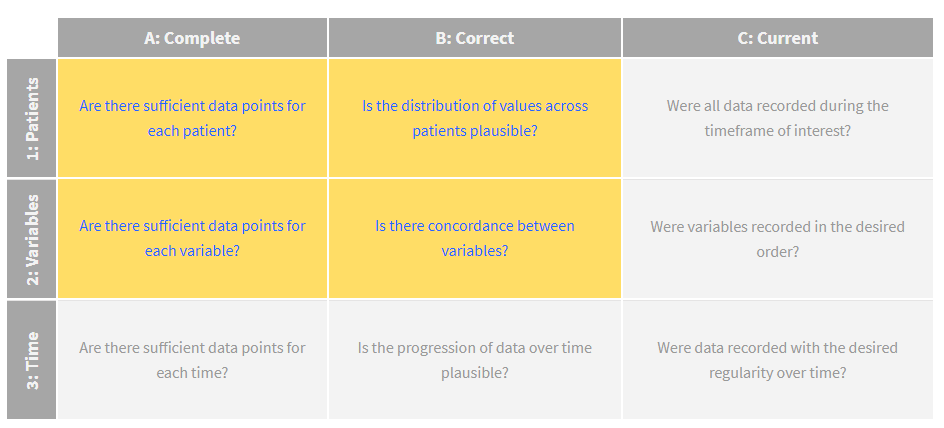
\includegraphics[width=15.5cm]{3x3Matrix.png}
		
		Für die Matrixfelder 1B und 2A soll exemplarisch der Qualitätsscore gemäß der Empfehlung von Weiskopf \textit{et al.}~\cite{10.5334/egems.218} berechnet werden.
		\begin{description}
			\item 1B. The distribution of values across patients is plausible.\\
			Für die Berechnung des Qualitätsscores in diesem Matrixfeld muss zwischen diskreten und kontinuierlichen Variablen unterschieden werden. Für die diskreten Variablen werden mögliche Werte im folgenden absolut festgelegt, für kontinuerliche Variablen wird der erlaubte Wertebreich relativ festgelegt. Hierbei wird sich an Boxplots orientiert und die Werte außerhalb der Whisker (unteres Limit: unteres Quartil subtrahiert um das 1,5-fache des Interquartilsabstands, oberes Limit: oberes Quartil addiert um das 1,5-fache des Interquartilsabstandes) werden als unplausibel angesehen.
			Zeitwerte werden hierbei außer Acht gelassen, da sie innerhalb anderer Matrixfelder Beachtung fänden.
			Somit ergeben sich folgende Scores für die genannten Variablen:\par			
			\textbf{SCTID:365581002 | Finding of marital or partnership status (finding):} Hierbei handelt es sich um eine diskrete Variable. Mögliche Werte sind SCTID:87915002 (Married (finding)), SCTID:125681006 (Single person (finding)) und SCTID:160504008 (Marital state unknown (finding)).
			In dem Datenset, das 498 Zeilen enthält, von denen 495 nicht leer sind, befinden sich alle Werte der Variable Finding of marital or partnership status (finding) innerhalb des Wertebereichs. Der Qualitätsscore für diese Variable beträgt somit 100~\%.\par
			\textbf{SCTID:372148003 | Ethnic group (ethnic group):} Hierbei handelt es sich um eine diskrete Variable. Mögliche Werte sind SCTID:315280000 (Asian - ethnic group (ethnic group)), SCTID:315240009 (Black - ethnic group (ethnic group)), SCTID:66920001 (Amerind (ethnic group)) und SCTID:185984009 (White - ethnic group (ethnic group)).
			Bereits beim Mapping sind die Werte "w" und "Alien" aufgefallen, die nicht innerhalb des erwarteten Wertebereichs liegen.
			In dem Datenset, das 498 Zeilen enthält, von denen 495 nicht leer sind, befinden sich 480 innerhalb des Wertebereichs. Der Qualitätsscore für diese Variable beträgt somit 96,97~\%.\par
			\textbf{SCTID:365873007 | Gender finding (finding):} Hierbei handelt es sich um eine diskrete Variable. Mögliche Werte sind SCTID:703118005 (Feminine gender (finding)) und SCTID:703117000 (Masculine gender (finding)). In dem Datenset, das 498 Zeilen enthält, von denen 495 nicht leer sind, befinden sich alle Werte der Variable Finding of marital or partnership status (finding) innerhalb des Wertebereichs. Der Qualitätsscore für diese Variable beträgt somit 100~\%.\par
			\textbf{LOINC VALUE:} Hierbei handelt es sich um eine heterogene Gruppe von Laborwerten und damit teils um kategoriale, teils um kontinuierliche Messwerte. Jeder LOINC CODE steht für eine unterschiedliche Variable. Beim LOINC CODE 72166-2 (Tobacco smoking status NHIS
			) handelt es sich beispielsweise um eine diskrete Variable, während es sich beim LOINC CODE 2708-6 (Oxygen saturation in Arterial blood) um eine kontinuierliche Variable handelt.
			Der Qualitätsscore soll für die gesamte Spalte berechnet werden, für jeden LOINC CODE wird je die Zahl von unplausiblen Variablen bestimmt und anschließend ein Gesamtscore berechnet. Zunächst fällt auf, dass von den 495 nicht-leeren Zeilen des Datensatzes 151 Zeilen für die Variable LOINC Value Daten des Datentyps Datum enthalten, die nicht dem erwarteten Wertebereich entsprechen. Somit qualifizieren sich lediglich 69,5~\% der Werte für eine nähere Betrachtung. Alle diskreten Variablen befinden sich jeweils im erwarteten Wertebereich. Für die Betrachtung der kontinuierlichen Variablen werden zunächst die Zeilen, die den Datenyp als LOINC VALUE enthalten, manuell aus dem Datensatz entfernt und dieser wird unter dem Dateinamen \textsf{Hausarbeit\_Datensatz\_COVID19\_LK\_v1.5.xlsx} abgespeichert und in den FAIRDOMHub geladen. Über ein Python Skript wird nun je ein Boxplot für die Werteverteilung innerhalb eines LOINC CODE oder einer SCTID:273249006 (Asessment Scale) erstellt und die Ausreißer werden visuell abgelesen. Das Skript ist im GitHub-Repositorium verfügbar (\url{https://raw.githubusercontent.com/lknegendorf/Master-BIDS-FDM_Hausarbeit/main/DataQuality.py}). Exemplarisch ist in Abbildung 2.1 der Boxplot für den LOINC CODE 8302-2 dargestellt, alle Boxplots befinden sich im Anhang dieser Hausarbeit.
			\begin{figure}
				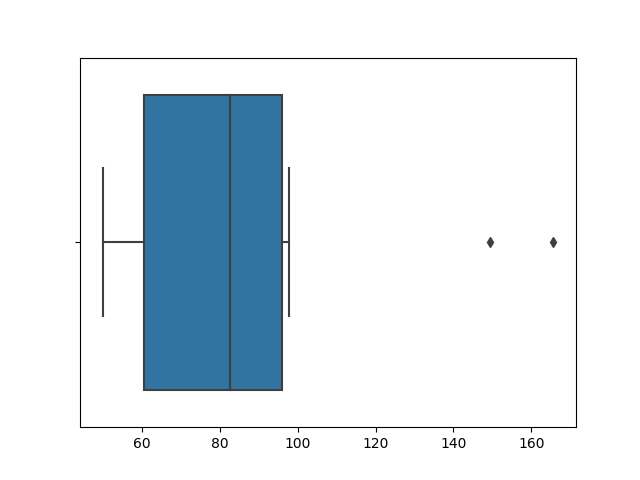
\includegraphics[width=15.5cm]{Graphs/8302-2.png}
				\caption{Verteilung des Wertebreichs für LOINC CODE 8302-2}
			\end{figure}
		 	Durch visuelles Ablesen der erzeugten Boxplots ergeben sich 12 Ausreißer nach oben definierten Kriterien, diese treten bei folgenden LOINC CODES auf: 777-3, 8302-2, 8462-4, 8480-6, 9279-1, 29463-7. Für den LOINC CODE 704-7 und den SCTID:273249006 sind zu wenige Werte repräsentiert, dass ein sinnhafter Boxplot entsteht. Die auftretenden Ausreißer werden bei letzteren beiden als sinnhafte Werte gezählt.
		 	Insgesamt beträgt der Qualitätsscore für diese Variable somit 67,07~\%.\par
			
			\item 2A. There are sufficient data for each variable.\\
			Für die Berechnung des Qualitätsscores in diesem Matrixfeld muss die Werteverteilung über die Zeit und über verschiedene Patienten betrachtet werden. Da es, wie weiter oben beschrieben, leider nicht möglich ist, einzelne Patienten im Datenset zu identifizieren, kann dieses Matrixfeld nicht wie von Weiskopf \textit{et al.} geprüft werden. Deswegen wird hierfür auf die Anzahl der Werte für Variablen rekurriert und hier eine annähernde Plausibilität geprüft.
			In dem Datenset, das 498 Zeilen enthält, sind 3 Zeilen leer, enthalten also keine Werte. Es ist unklar, ob dieser Umstand lediglich durch einen Formatierungsfehler oder durch tatsächlich verlorengegangene Werte entstanden ist. Sollte es sich um verlorengegangene Werte handeln, mindert dieser Umstand den Qualitätsscore in diesem Matrixfeld bereits um 0,6~\%.
			Im folgenden wird kurz für jede Variable, für die nicht 495 Werte definiert sind, begründet, ob dieser Umstand plausibel ist. Eine genaue Berechnung des Qualitätsscores kann aus geannten gründen nicht erfolgen.\par
			\textbf{SCTID:399753006 | Date of death (observable entity):} Es sind für 70 von 495 Zeilen Werte definiert, dies entspricht 14,14~\%. Dieser Umstand wird als plausibel angesehen, da ein Todesdatum nur angegeben werden kann, wenn ein Patient bereits verstorben ist. Orientierend lässt sich anhand der Geburtsdaten feststellen, dass viele Patienten innerhalb einer normalen Lebenserwartung liegen.\par
			\textbf{LOINC UNITS:} Es sind für 431 von 495 Zeilen Werte definiert, dies entspricht 87,07~\%. Die undefinierten Werte treten ausschließlich bei den diskreten Variablen auf, deswegen ist dieser Umstand plausibel.\par
			\textbf{Condition Stop Date (SCTID:410672004 | Date property (qualifier value)):} Es sind für 309 von 495 Zeilen Werte definiert, dies entspricht 62,42~\%. Es ist ohne weitere Kenntnis der Umstände oder ohne Möglichkeit, in die Patientenakten zu schauen, sehr schwierig, eine Plausibilität zu prüfen. Beim überwiegenden Teil der Zeilen, für die kein Wert angegeben ist, handelt es sich um Conditions, die chronischen Krankheiten entsprechen, was den Umstand der fehlenden Werte plausibel macht. Bei bestimmten Conditions wie z.B. Cardiac Arrest oder Atrial Fibrillation ist aus medizinischer Sicht zu diskutieren, ob es plausibel ist, dass kein Enddatum angegeben wird.\par
			\textbf{Medication Stop Date (SCTID:410672004 | Date property (qualifier value)):} Es sind für 428 von 495 Zeilen Werte definiert, dies entspricht 86,46~\%. Es ist plausibel, dass Patienten in einem solchen Anteil Medikamente auf Lebenszeit einnehmen.\par
			\textbf{Medication Reason:} Es sind für 418 von 495 Zeilen Werte definiert, dies entspricht 84,44~\%. Jede Verordnung eines Medikamentes sollte aus medizinischer Sicht einen Grund haben, weswegen es sich hier am ehesten um fehlende Werte handelt, die die Vollständigkeit des Datensatzes beeinträchtigen.
		\end{description}
		Der Qualitätsscore wird stark negativ durch die Datumswerte im Abschnitt Observations beeinflusst. Es ist unklar, wie diese entstanden sind. Es könnte sich um einen Formatfehler in Excel handeln, sodass aus einem numerischen Wert von beispielsweise 21.3 durch das Datum 21.03.2021 entsteht. Leider ist dieser Umstand im Datensatz aber nicht mehr nachvollziehbar, sodass aufgrund von Integritätsüberlegungen diese Annahme nicht einfach umgesetzt werden kann. Um den Score zu verbessern, bleibt somit nur, zunächst alle Zeile mit Datumswerten zu entfernen. Dies wurde in der oben beschriebenen Datensatzversion 1.5 bereits umgesetzt. Weitere Verbesserungen werden durch ein entfernen der Leerzeilen, sowie ein Entfernen aller oben beschriebenen Datensätze mit Ausreißerwerten erreicht. Da aufgrund der Forschungsfrage des Beispielszenarios nur die Medikationen von Patienten interessant sind und nicht die Gründe für eine Medikation, werden die Spalten zur Medication Reason gelöscht, um auch hier eine Verbesserung des Scores zu erreichen. Die Umsetzung der Verbesserungen geschieht händisch in Excel.
		Nach Beendingung der hier beschriebenen Bearbeitungen wird der Datensatz mit dem Dateinamen in den FAIRDOMHub geladen. Hierbei handelt es sich um folgenden Datensatz:\par
		\textsf{Hausarbeit\_Datensatz\_COVID19\_LK\_v2.xlsx,  \url{https://sandbox12.fairdomhub.org/data_files/54?version=5}, Checksummen: 999e95d52bb9a7d59b1e0ae4a331e917~(MD5), 4382cc970686895bfe64a729520115027220960c1981da64fd7e99c309948a9b~(SHA256)}
	
		\section*{3. Meta-Daten}
		Im folgenden soll der vorliegende Datensatz durch Metadaten ergänzt werden. Während des bisherigen Bearbeitungsprozesses sind bereits zwei verschiedene Metadatentypen auf Ebene der Datenitems ergänzt worden: Einerseits die Umbenennung der Spalten mit einem Mapping auf die entprechenden SNOMED CT und LOINC Bezeichnungen, andererseits die Umsetzung eines Mappings der Variablen für die Spalten SCTID:365581002 (Finding of marital or partnership status (finding)), SCTID:372148003 (Ethnic group (ethnic group)), SCTID:365873007 (Gender finding (finding)), und SCTID:273249006 (Assessment scales (assessment scale)).
		Erstere Maßnahme wurde getroffen, da die Variablen bereits in der entsprechenden Terminologie SNOMED CT, LOINC oder RxNorm vorlagen. Hier war es lediglich notwendig, auch auf diese Terminologien zu verweisen, damit der Bezug eindeutig ist und die Daten maschinenlesbar werden. Das Mapping der Variablen auf bestehende SNOMED CT Terme wurde durchgeführt, um dem Interoperabilitätskriterium der FAIR-Kriterien gerecht zu werden. SNOMED CT wurde ausgewählt, da es sich hierbei um einen international verbreiteten und anerkannten Standard handelt.\par
		Bisher wurden die Variablen der Spalten SCTID:169812000 (Place of birth (observable entity)) und DISPENSES, noch nicht durch Metadaten beschrieben, da für erstere kein einfach zu mappendes standardisiertes Format möglich war und für zweiteres kein Term in den bereits verwendeten Terminologien vorhanden war. Der Datentyp der Variablen für die Spalte SCTID:169812000 wird in den Metadaten eigens definiert auf \textsf{<CityName:string>\~{}\~{}<StateName:string>\~{}\~{}<countryCode:ISO 3166-1 alpha-2>}, wobei die Tilde für ein Leerzeichen steht. Der Inhalt der Spalte DISPENSES muss mit Text erklärt werden: 'Anzahl der verschriebenen Dosen des Medikamentes', der Datentyp ist \textsf{integer}.
		Für die Ergänzung von Metadaten auf Ebene des Datensatzes wird das DataCite XML-Schema verwendet (\url{https://schema.datacite.org/}). DataCite ist eine Plattform, die Ressourcen aus verschiedenen Repositorien enthält, weswegen ein guter Grad an Standardisierung vorliegt. Das XML Format ermöglicht neben einer weiteren Standardisierung auch eine Maschinenlesbarkeit der Metadaten auf Ebene des Datensatzes. Für die Erstellung der Metadaten auf Datensatzebene nach dem gewählten Schema fehlt allerdings noch die zwingend anzugebende DOI, weswegen diese Metadaten zunächst als vorläufig markiert werden müssen.
		Die ersten drei angegebenen Metadatentypen werden in einer Tabelle in Markdown-Language zusammengefasst und zusammen mit dem Datensatz und dem XML Schema in den FAIRDOMHub geladen. Der Datensatz selbst wurde in diesem Schritt nicht bearbeitet und wird gemäß Aufgabenstellung unverändert als neue Version in den FAIRDOMHub geladen. Ebenso werden die Metadaten hochgeladen. Hierbei handelt es sich um folgenden Datensatz:\par
		\textsf{Hausarbeit\_Datensatz\_COVID19\_LK\_v3.xlsx,  \url{https://sandbox12.fairdomhub.org/data_files/54?version=6}, Checksummen: 999e95d52bb9a7d59b1e0ae4a331e917~(MD5), 4382cc970686895bfe64a729520115027220960c1981da64fd7e99c309948a9b~(SHA256)}    
	
		\section*{4. Datenaufbereitung}
		Im Folgenden wird der Datensatz final bereinigt, bevor er veröffentlicht wird. Bezüglich der Plausibilität fällt als erstes auf, dass es Zeilen gibt, die in der Spalte Observation Date (SCTID: 410672004 Date property (qualifier value)) keine Daten des Typs Datum enthalten, sondern unplausible Zahlwerte, diese Zeilen werden entfernt. Weiterhin fällt auf, dass die Spalte SCTID: 169812000 Place of birth (observable entity) Werte mit nicht-druckbaren Zeichen enthält. Dies betrifft den Eintrag der Stadt Hanoi. Da unklar ist, welche Zeichen dieses Datenitem ursprünglich enthielt, wird die Zeile aus den Daten entfernt. Es wird nach Duplikaten gesucht, allerdings werden keine doppelten Zeilen gefunden (diese wurden bereits in Schritt 2 entfernt, da sie ebenfalls Werte schlechter Datenqualität enthielten). Zuletzt wird in der Spaltenbeschriftung jeweils das | Zeichen entfernt, da dieses problematisch bei der eindeutigen Bezeichnung der Spalten in mit Markdown erstellten Tabellen ist. Außerdem wird die erste Spalte, die Reihenindizes aus einem vorangegangenen Python Export enthält, welche nicht im ursprünglichen Datensatz vorhanden waren, gelöscht. Zusätzlich wird die Spalte PATIENTS gelöscht, da sie wie oben beschrieben in der Bearbeitung der Hausarbeit keine Beachtung gefunden hat. Der Datensatz wird in der aktualisierten Version in den FAIRDOMHub geladen und das Metadaten-Schema der Datenitems wird entsprechend angepasst, damit es wieder eindeutig auf den Datensatz referenziert. Beim zuletzt hochgeladenen Datensatz handelt es sich um folgenden:\par
		\textsf{Hausarbeit\_Datensatz\_COVID19\_LK\_v4.xlsx,  \url{https://sandbox12.fairdomhub.org/data_files/54?version=7}, Checksummen: 58a5774f7a753e03c8537ea1cd7b89b5~(MD5), c7e7489ffd4eb73dc1c50f5e724b752adf174010f8188139349d1ef4fa801f64~(SHA256)}
	
		\section*{5. Datenpublikation}
		Der Datensatz in der oben genannten Version wird auf der Plattform Zenodo unter dem \doi{10.5281/zenodo.4668732} publiziert. Die Wahl der Plattform Zenodo erfolgte aus mehreren Gründen. Einerseits ist es rein praktisch möglich, den DOI bereits vor finaler Veröffentlichung des Datensatzes zu reservieren. Dies ermöglichte es, den DOI in den Metadaten zu inkludieren und damit die Matdaten gemäß den FAIR Kriterien korrekt auf den Datensatz zu referenzieren. Außerdem ist Zenodo eine sehr offene Plattform, die eine Reihe von Formaten erlaubt und wenige Minimalinformationen benötigt.
		Die Wahl der Lizenz erfolgte möglichst offen. Da die Hausarbeit selbst und die verschiedenen Bearbeitungsstufen im FAIRDOMHub bereits unter eine CC BY-SA 4.0 Lizenz erfolgten, wurde für die finale Version des veröffentlichten Datensatzes eine CC BY 4.0 Lizenz ausgewählt, um eine noch flexiblere Nachnutzung zu erlauben.
	
	\clearpage
	\singlespacing
	\bibliography{FDM_Hausarbeit-Literatur}
	\clearpage
				
	\chapter{Anhang}
		\section{Übersicht über Dateistruktur und Versionierung}
			\url{https://github.com/lknegendorf/Master-BIDS-FDM_Hausarbeit/wiki/%C3%9Cbersicht-%C3%BCber-Dateistruktur-und-Versionierung}
		\section{Checksummen Übersicht Datensatz}
			\url{https://github.com/lknegendorf/Master-BIDS-FDM_Hausarbeit/wiki/Checksummen-%C3%9Cbersicht-Datensatz}
		\section{Mapping Tabellen FAIR Kriterien I1}
			\url{https://github.com/lknegendorf/Master-BIDS-FDM_Hausarbeit/wiki/Mapping-Tabellen-FAIR-Kriterien-I1}

		\section{Boxplots zu einzelnen LOINC CODES im Datensatz}
			\begin{center}
			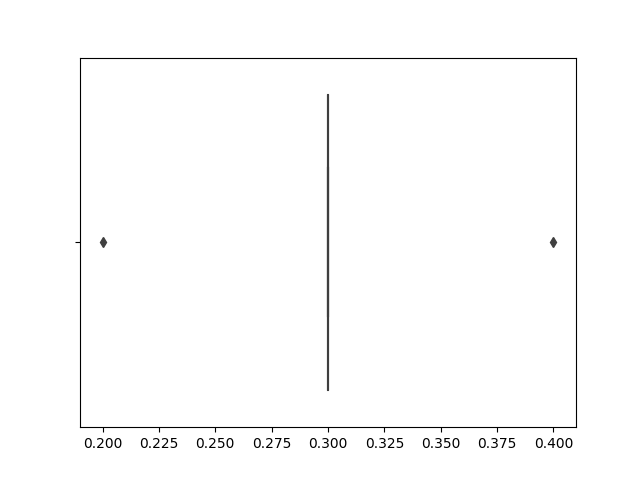
\includegraphics[width=8cm]{Graphs/704-7.png}
			
			\small{Verteilung des Wertebreichs für LOINC CODE 704-7}
			
			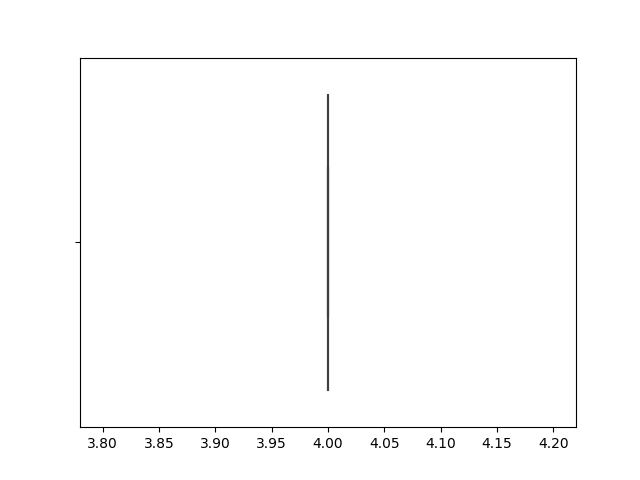
\includegraphics[width=8cm]{Graphs/706-2.png}
			
			\small{Verteilung des Wertebreichs für LOINC CODE 706-2}
			
			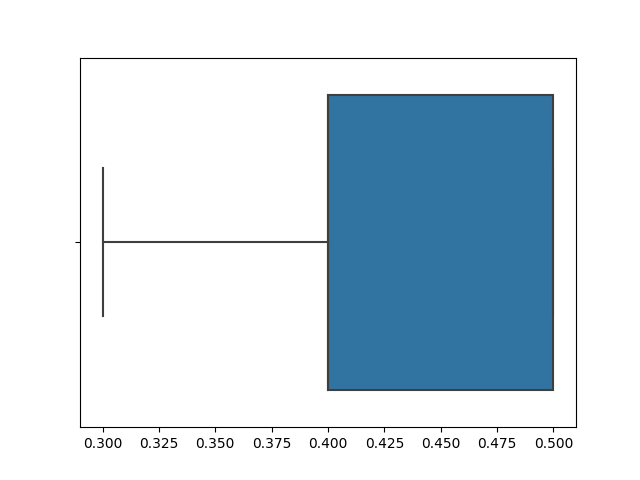
\includegraphics[width=8cm]{Graphs/711-2.png}
			
			\small{Verteilung des Wertebreichs für LOINC CODE 711-2}
			
			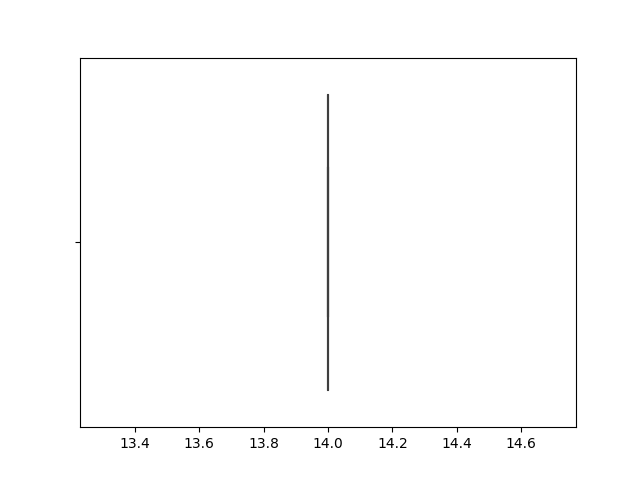
\includegraphics[width=8cm]{Graphs/718-7.png}
			
			\small{Verteilung des Wertebreichs für LOINC CODE 718-7}
			
			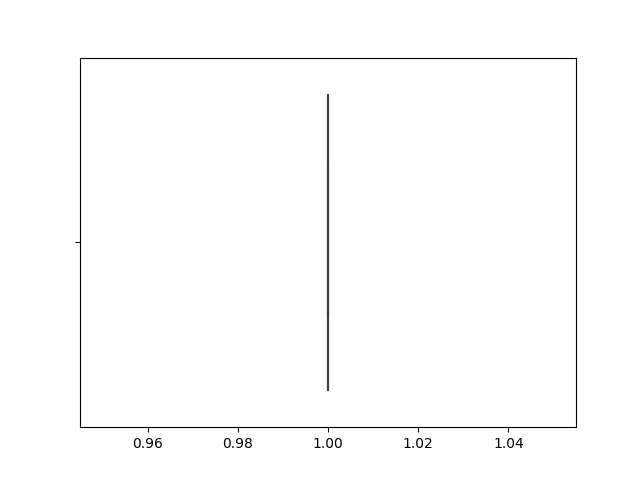
\includegraphics[width=8cm]{Graphs/731-0.png}
			
			\small{Verteilung des Wertebreichs für LOINC CODE 731-0}
			
			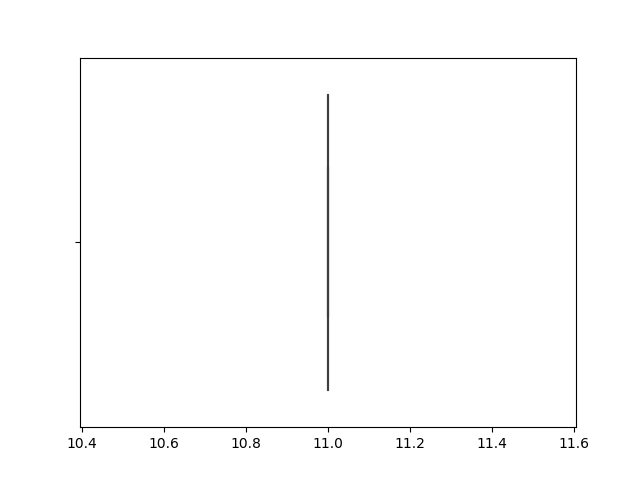
\includegraphics[width=8cm]{Graphs/736-9.png}
			
			\small{Verteilung des Wertebreichs für LOINC CODE 736-9}
			
			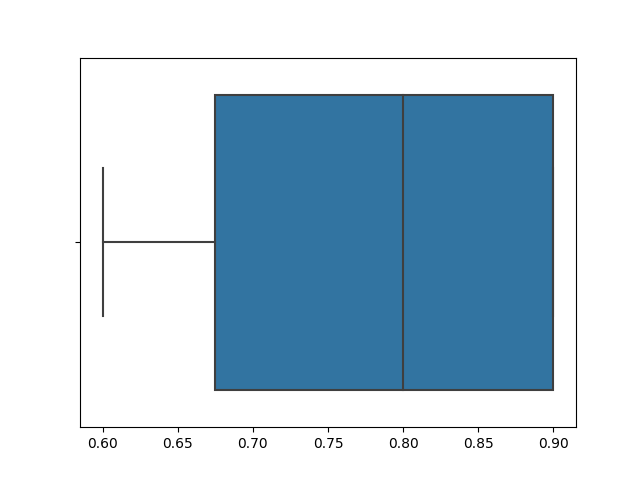
\includegraphics[width=8cm]{Graphs/742-7.png}
			
			\small{Verteilung des Wertebreichs für LOINC CODE 742-7}
			
			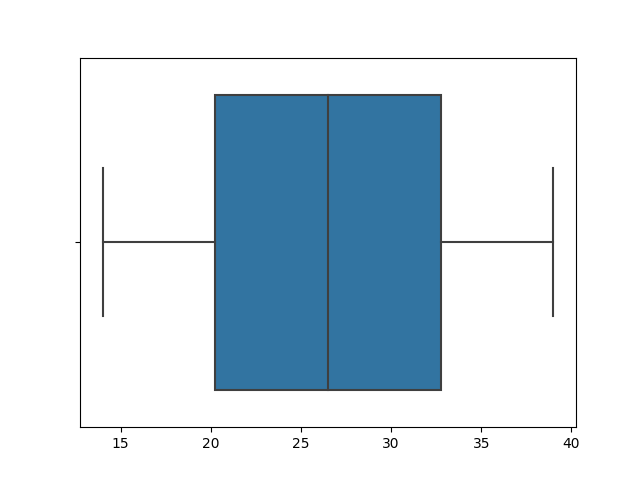
\includegraphics[width=8cm]{Graphs/770-8.png}
			
			\small{Verteilung des Wertebreichs für LOINC CODE 770-8}
			
			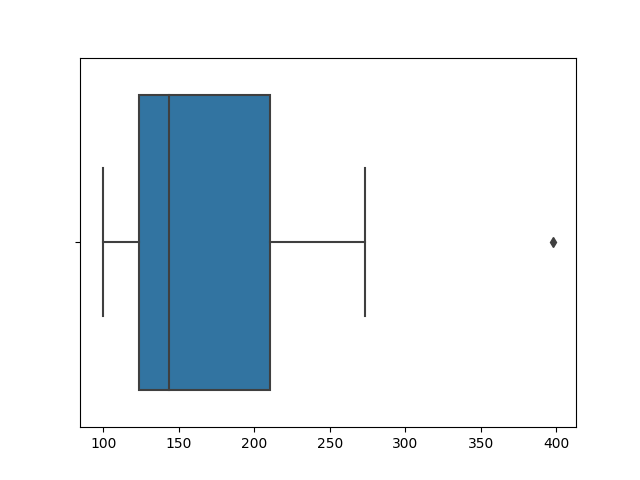
\includegraphics[width=8cm]{Graphs/777-3.png}
			
			\small{Verteilung des Wertebreichs für LOINC CODE 777-3}
			
			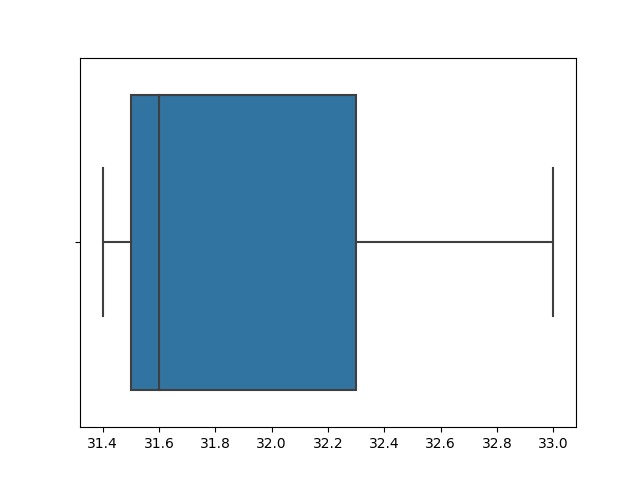
\includegraphics[width=8cm]{Graphs/785-6.png}
			
			\small{Verteilung des Wertebreichs für LOINC CODE 785-6}
			
			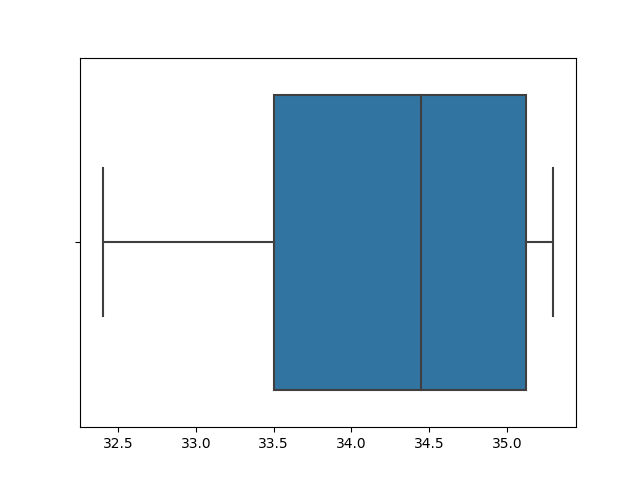
\includegraphics[width=8cm]{Graphs/786-4.png}
			
			\small{Verteilung des Wertebreichs für LOINC CODE 786-4}
			
			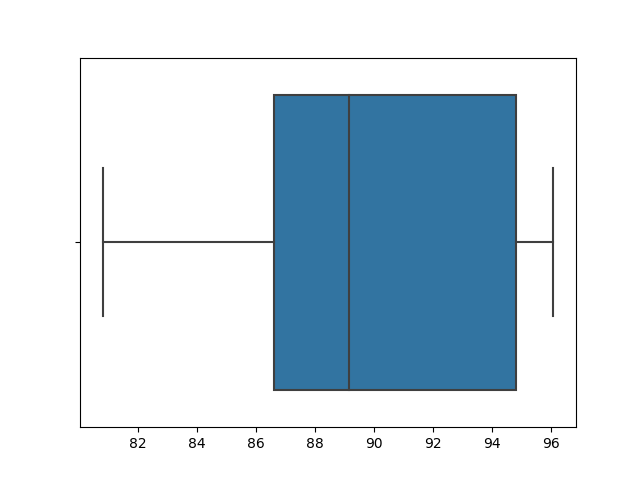
\includegraphics[width=8cm]{Graphs/787-2.png}
			
			\small{Verteilung des Wertebreichs für LOINC CODE 787-2}
			
			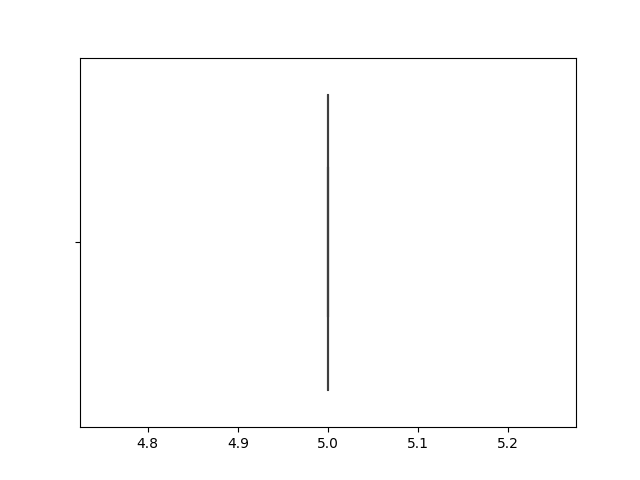
\includegraphics[width=8cm]{Graphs/789-8.png}
			
			\small{Verteilung des Wertebreichs für LOINC CODE 789-8}
			
			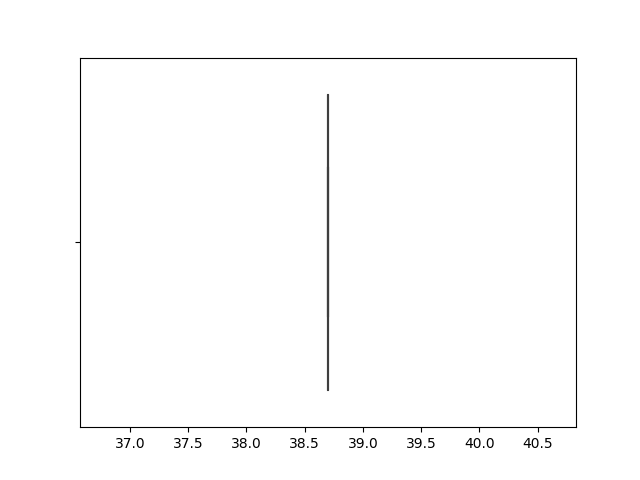
\includegraphics[width=8cm]{Graphs/1742-6.png}
			
			\small{Verteilung des Wertebreichs für LOINC CODE 1742-6}
			
			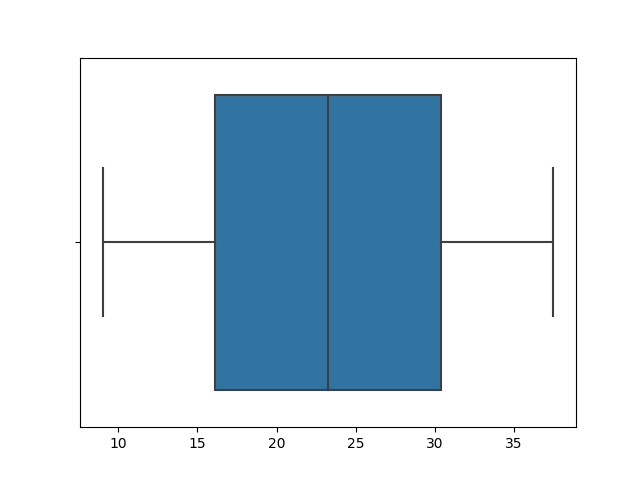
\includegraphics[width=8cm]{Graphs/1920-8.png}
			
			\small{Verteilung des Wertebreichs für LOINC CODE 1920-8}
			
			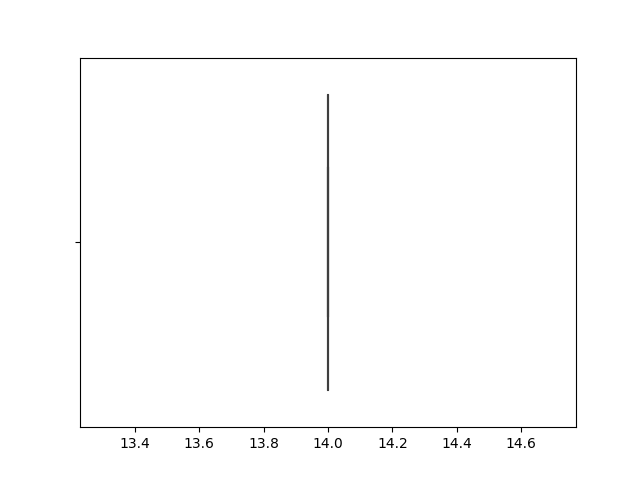
\includegraphics[width=8cm]{Graphs/1975-2.png}
			
			\small{Verteilung des Wertebreichs für LOINC CODE 1975-2}
			
			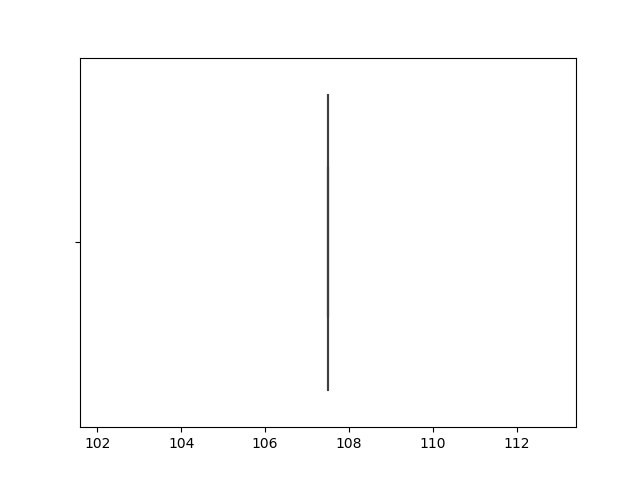
\includegraphics[width=8cm]{Graphs/2075-0.png}
			
			\small{Verteilung des Wertebreichs für LOINC CODE 2075-0}
			
			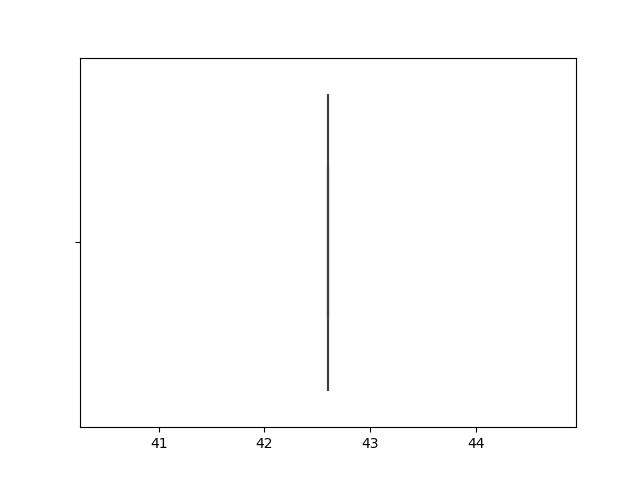
\includegraphics[width=8cm]{Graphs/2157-6.png}
			
			\small{Verteilung des Wertebreichs für LOINC CODE 2157-6}
			
			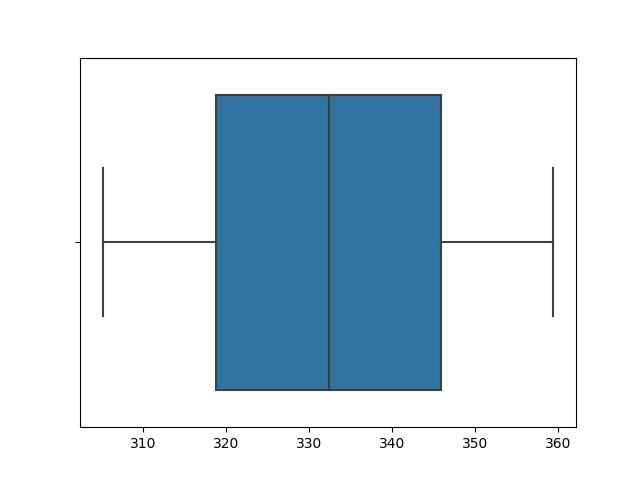
\includegraphics[width=8cm]{Graphs/2276-4.png}
			
			\small{Verteilung des Wertebreichs für LOINC CODE 2276-4}
			
			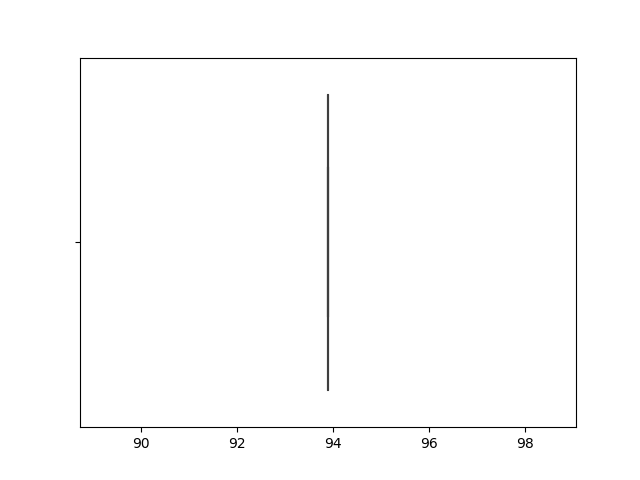
\includegraphics[width=8cm]{Graphs/2345-7.png}
			
			\small{Verteilung des Wertebreichs für LOINC CODE 2345-7}
			
			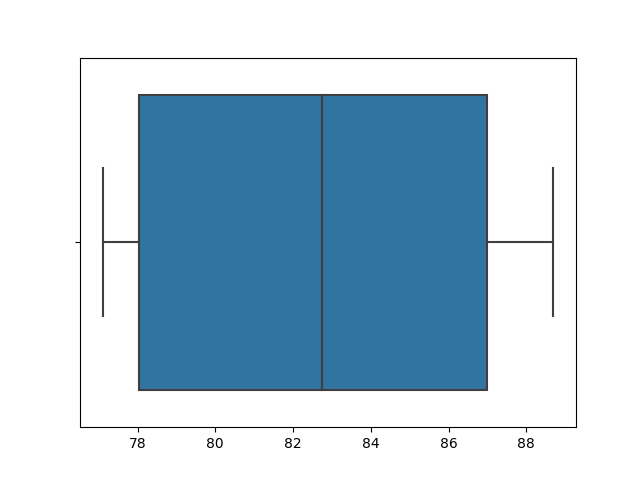
\includegraphics[width=8cm]{Graphs/2708-6.png}
			
			\small{Verteilung des Wertebreichs für LOINC CODE 2708-6}
			
			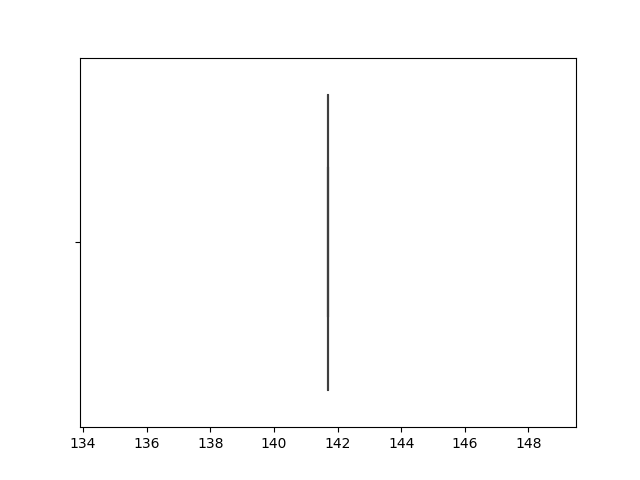
\includegraphics[width=8cm]{Graphs/2951-2.png}
			
			\small{Verteilung des Wertebreichs für LOINC CODE 2951-2}
			
			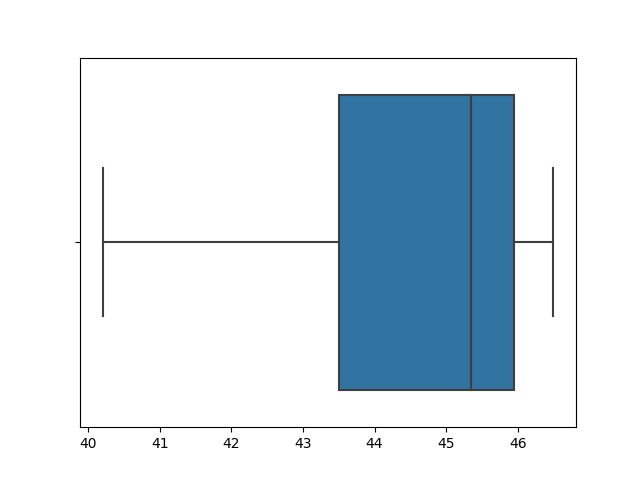
\includegraphics[width=8cm]{Graphs/4544-3.png}
			
			\small{Verteilung des Wertebreichs für LOINC CODE 4544-3}
			
			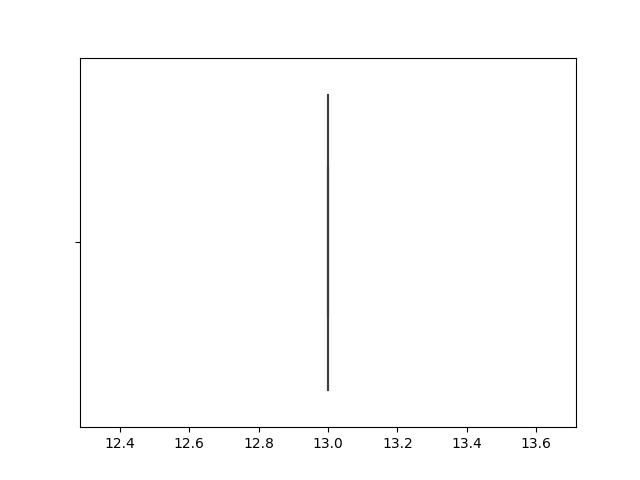
\includegraphics[width=8cm]{Graphs/5902-2.png}
			
			\small{Verteilung des Wertebreichs für LOINC CODE 5902-2}
			
			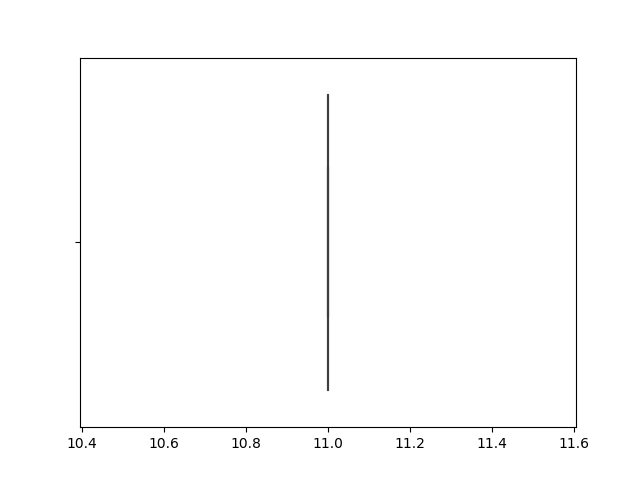
\includegraphics[width=8cm]{Graphs/5905-5.png}
			
			\small{Verteilung des Wertebreichs für LOINC CODE 5905-5}
			
			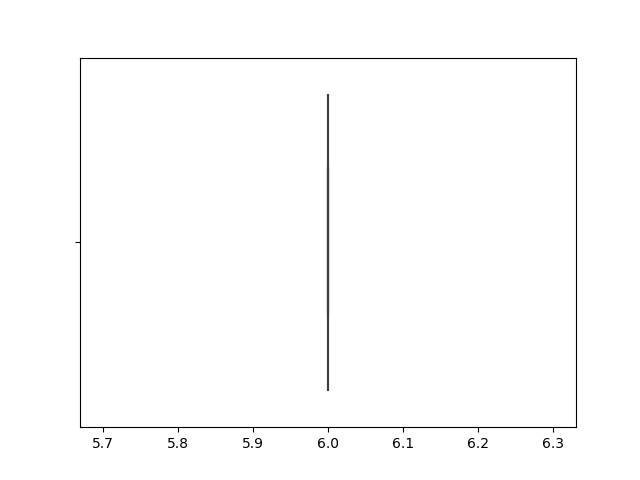
\includegraphics[width=8cm]{Graphs/6690-2.png}
			
			\small{Verteilung des Wertebreichs für LOINC CODE 6690-2}
			
			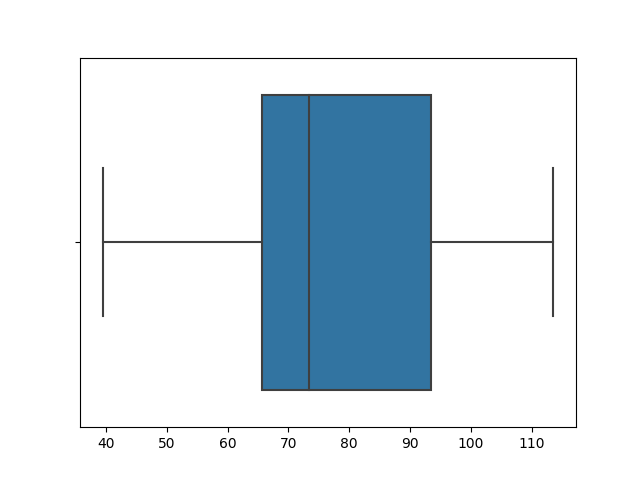
\includegraphics[width=8cm]{Graphs/6768-6.png}
			
			\small{Verteilung des Wertebreichs für LOINC CODE 6768-6}
			
			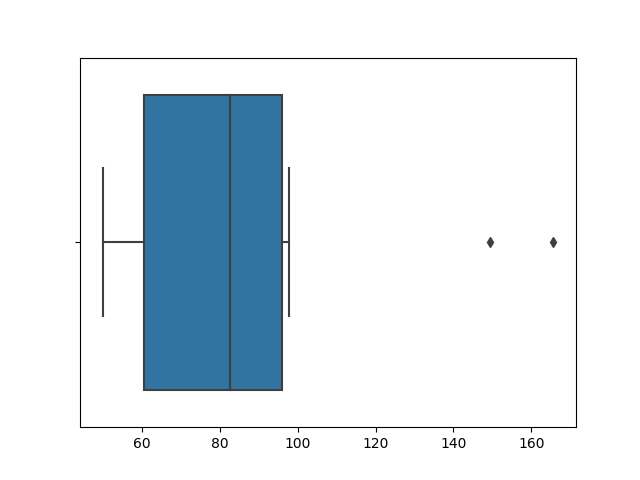
\includegraphics[width=8cm]{Graphs/8302-2.png}
			
			\small{Verteilung des Wertebreichs für LOINC CODE 8302-2}
			
			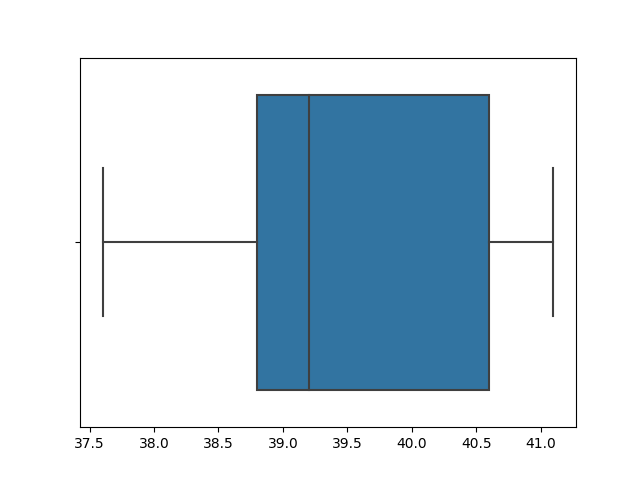
\includegraphics[width=8cm]{Graphs/8310-5.png}
			
			\small{Verteilung des Wertebreichs für LOINC CODE 8310-5}
			
			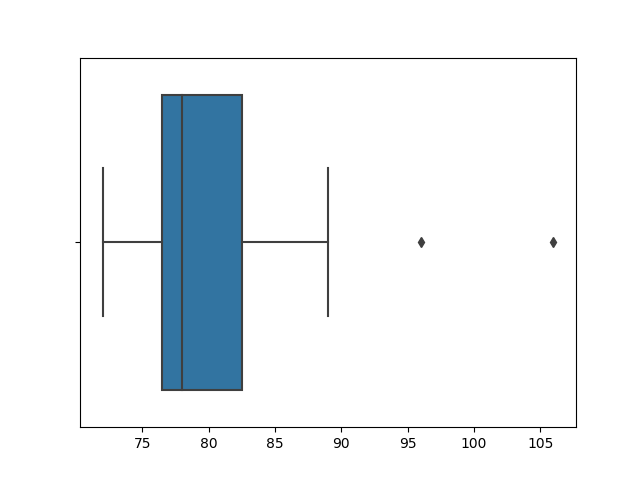
\includegraphics[width=8cm]{Graphs/8462-4.png}
			
			\small{Verteilung des Wertebreichs für LOINC CODE 8462-4}
			
			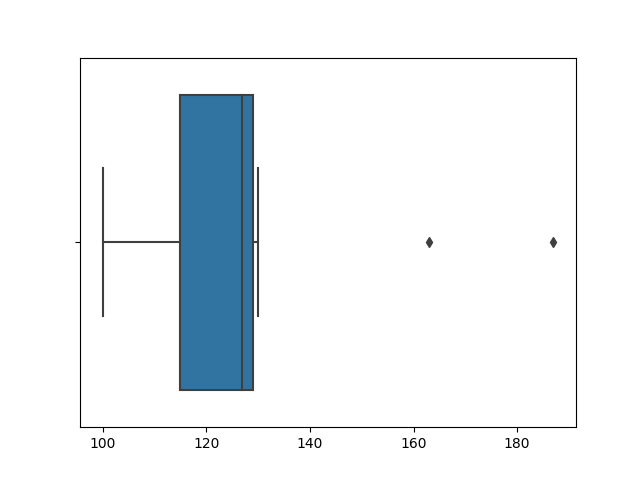
\includegraphics[width=8cm]{Graphs/8480-6.png}
			
			\small{Verteilung des Wertebreichs für LOINC CODE 8480-6}
			
			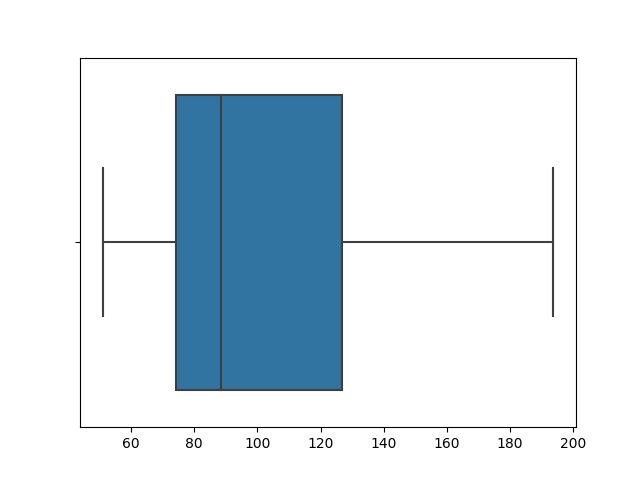
\includegraphics[width=8cm]{Graphs/8867-4.png}
			
			\small{Verteilung des Wertebreichs für LOINC CODE 8867-4}
			
			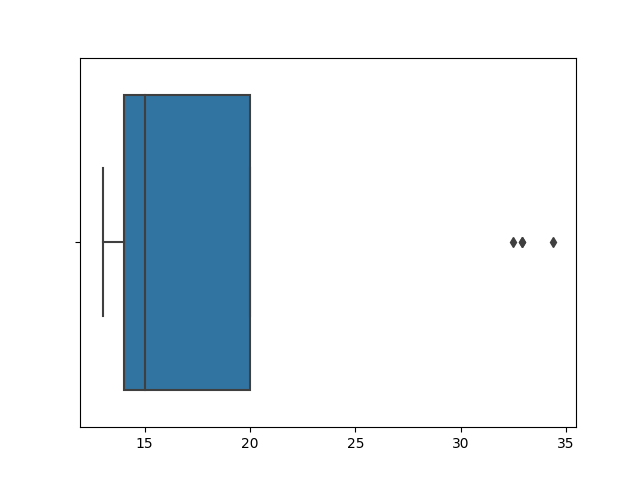
\includegraphics[width=8cm]{Graphs/9279-1.png}
			
			\small{Verteilung des Wertebreichs für LOINC CODE 9279-1}
			
			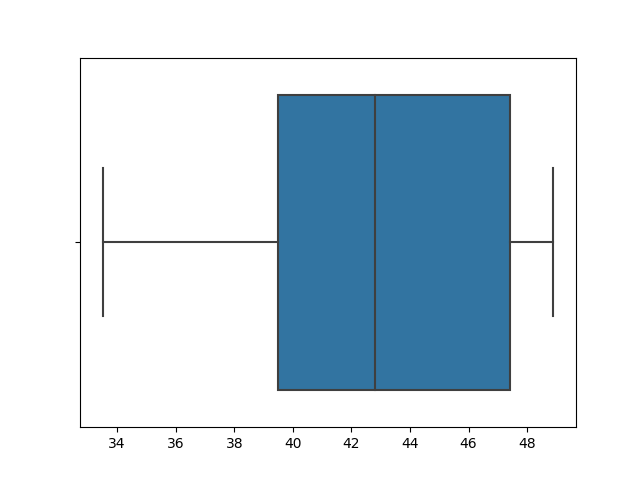
\includegraphics[width=8cm]{Graphs/9843-4.png}
			
			\small{Verteilung des Wertebreichs für LOINC CODE 9843-4}
			
			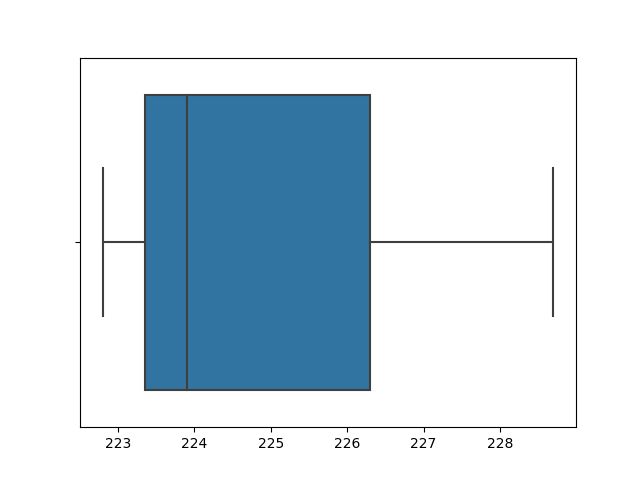
\includegraphics[width=8cm]{Graphs/14804-9.png}
			
			\small{Verteilung des Wertebreichs für LOINC CODE 14804-9}
			
			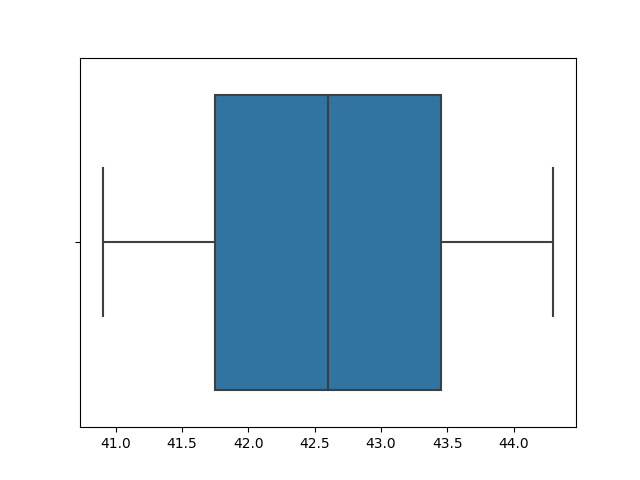
\includegraphics[width=8cm]{Graphs/21000-5.png}
			
			\small{Verteilung des Wertebreichs für LOINC CODE 21000-5}
			
			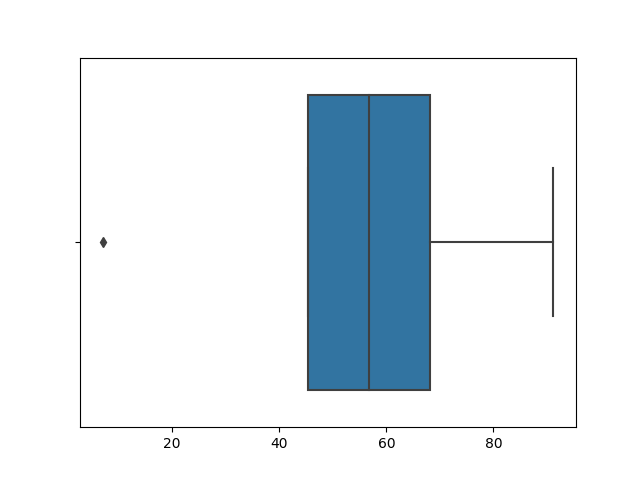
\includegraphics[width=8cm]{Graphs/29463-7.png}
			
			\small{Verteilung des Wertebreichs für LOINC CODE 29463-7}
			
			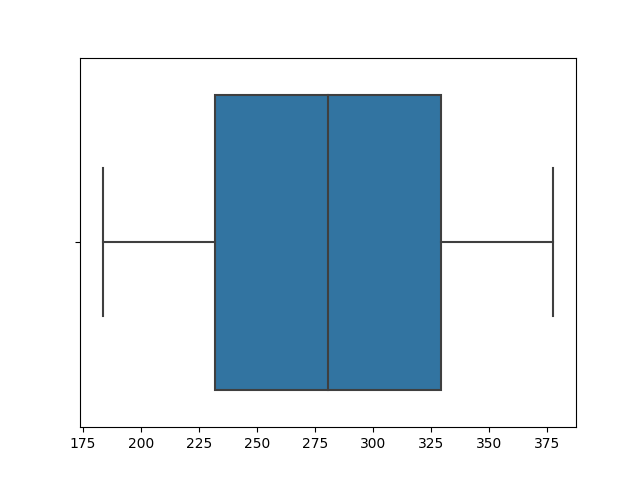
\includegraphics[width=8cm]{Graphs/32207-3.png}
			
			\small{Verteilung des Wertebreichs für LOINC CODE 32207-3}
			
			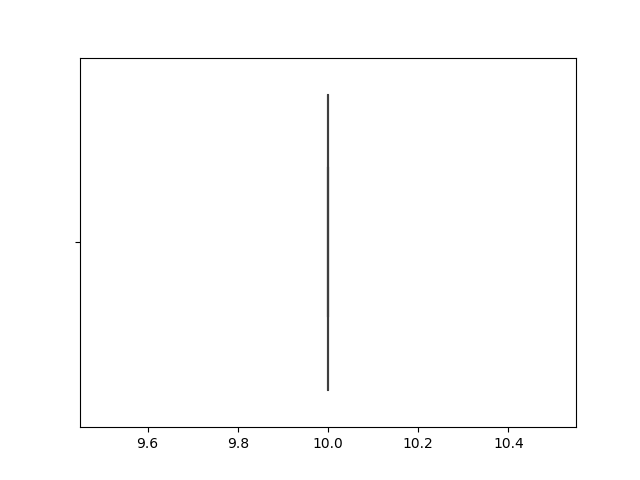
\includegraphics[width=8cm]{Graphs/33914-3.png}
			
			\small{Verteilung des Wertebreichs für LOINC CODE 33914-3}
			
			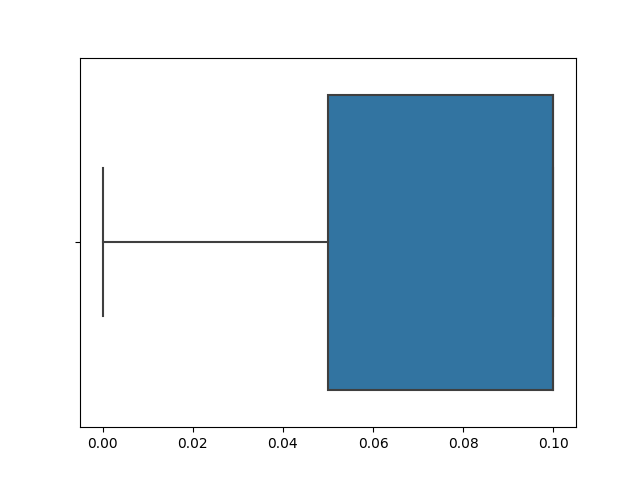
\includegraphics[width=8cm]{Graphs/33959-8.png}
			
			\small{Verteilung des Wertebreichs für LOINC CODE 33959-8}
			
			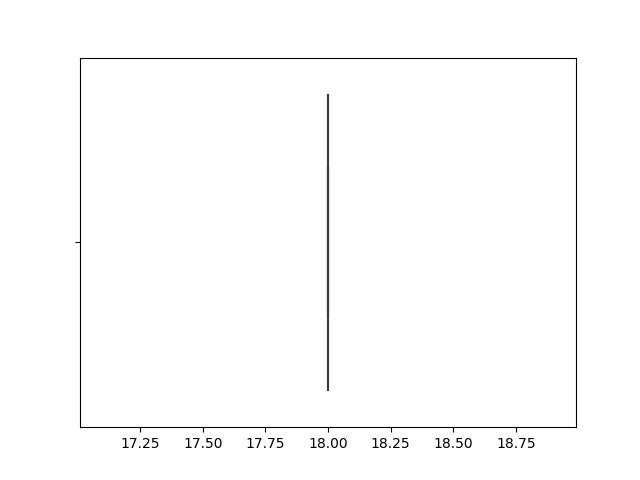
\includegraphics[width=8cm]{Graphs/39156-5.png}
			
			\small{Verteilung des Wertebreichs für LOINC CODE 39156-5}
			
			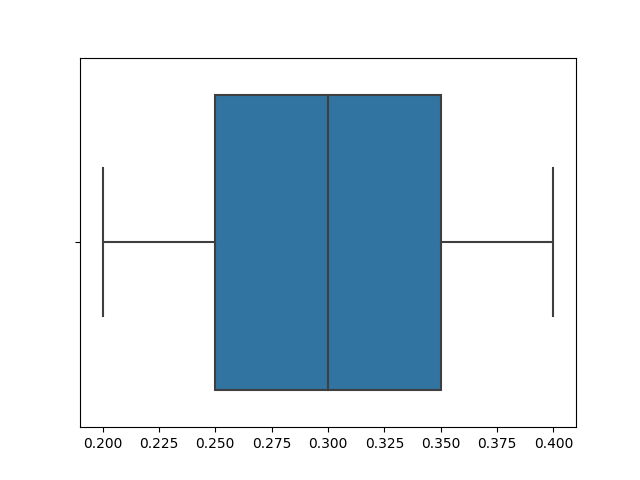
\includegraphics[width=8cm]{Graphs/48065-7.png}
			
			\small{Verteilung des Wertebreichs für LOINC CODE 48065-7}
			
			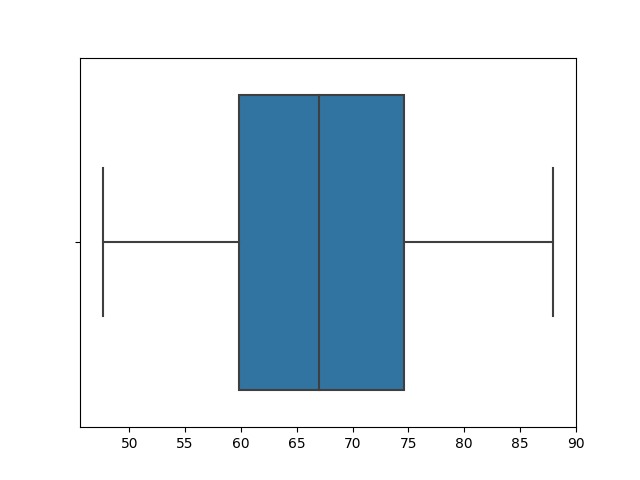
\includegraphics[width=8cm]{Graphs/59576-9.png}
			
			\small{Verteilung des Wertebreichs für LOINC CODE 59576-9}
			
			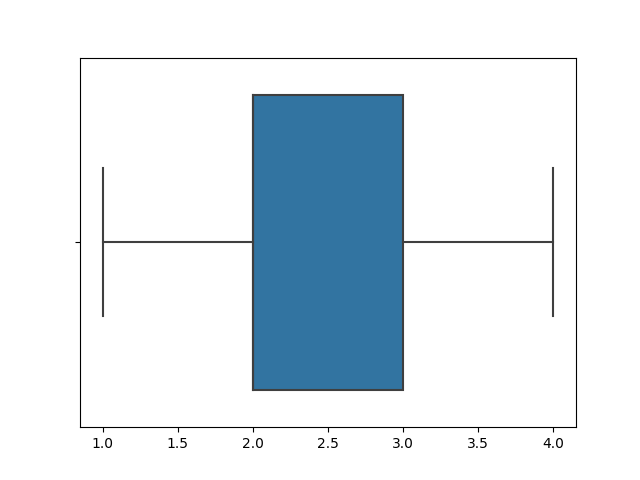
\includegraphics[width=8cm]{Graphs/72514-3.png}
			
			\small{Verteilung des Wertebreichs für LOINC CODE 72514-3}
			
			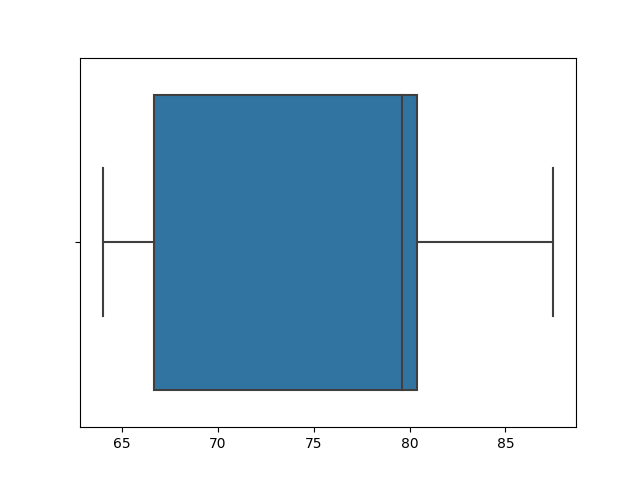
\includegraphics[width=8cm]{Graphs/77606-2.png}
			
			\small{Verteilung des Wertebreichs für LOINC CODE 77606-2}
			
			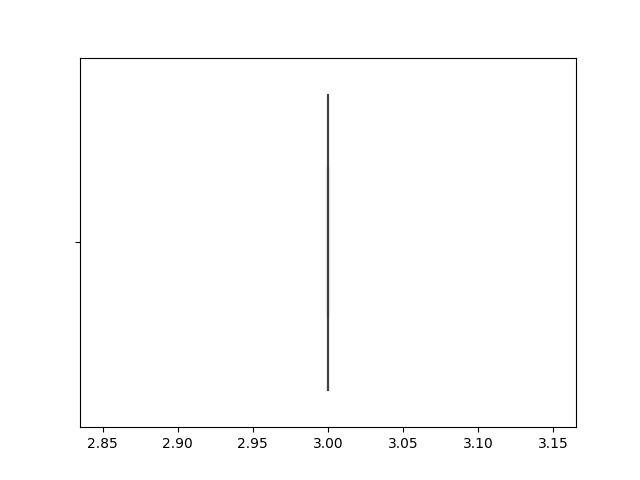
\includegraphics[width=8cm]{Graphs/89579-7.png}
			
			\small{Verteilung des Wertebreichs für LOINC CODE 89579-7}
			
			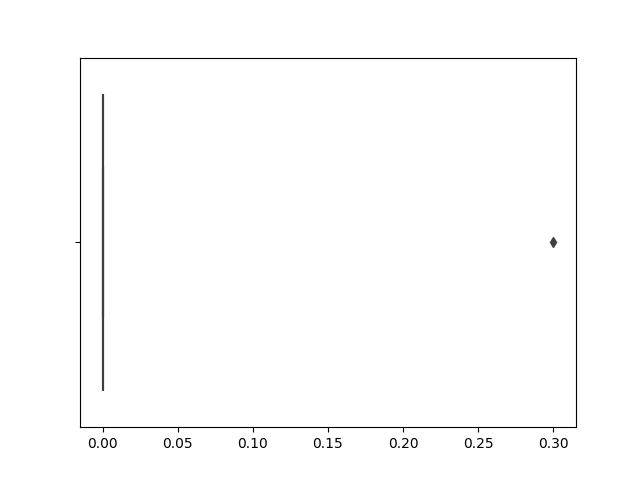
\includegraphics[width=8cm]{Graphs/273249006.png}
			
			\small{Verteilung des Wertebreichs für SCTID:273249006}
			
			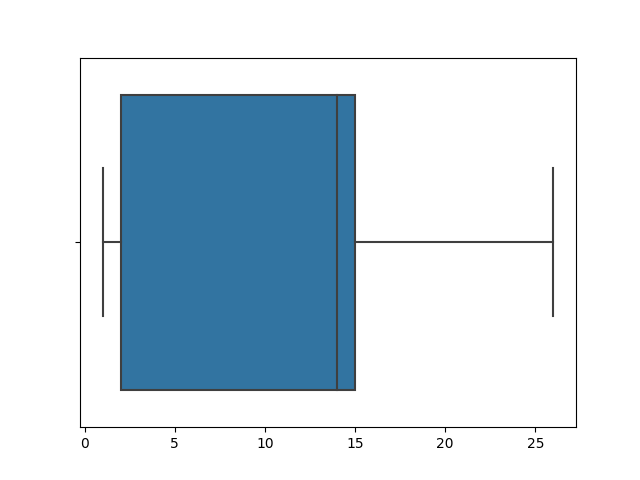
\includegraphics[width=8cm]{Graphs/273724008.png}
			
			\small{Verteilung des Wertebreichs für SCTID:273724008}
			
			\includegraphics[width=8cm]{Graphs/273725009.png}
			
			\small{Verteilung des Wertebreichs für SCTID:273725009}
			\end{center}
		\clearpage
\end{document}
